\documentclass[border=4pt]{standalone}
\usepackage{tikz}
\usetikzlibrary{shapes.symbols,shapes.geometric,positioning,arrows.meta}

\begin{document}
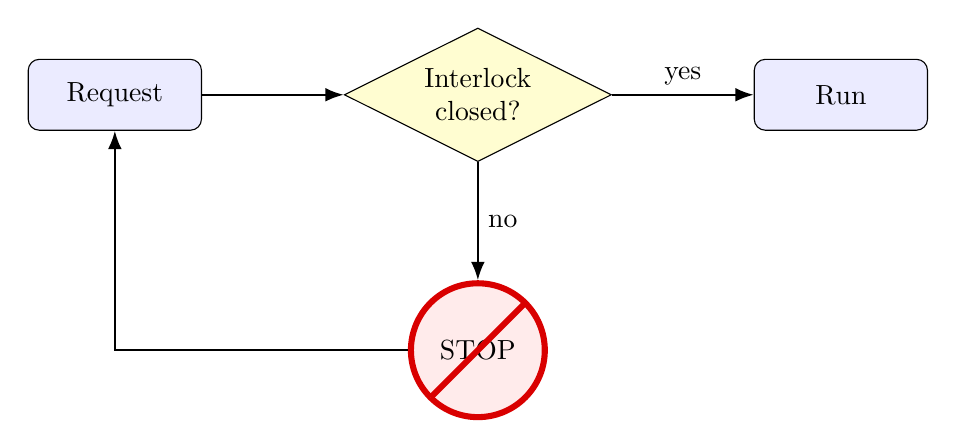
\begin{tikzpicture}[
  >=Latex,
  node distance=15mm and 18mm,
  block/.style={draw,rounded corners,minimum width=22mm,minimum height=9mm,fill=blue!8},
  gate/.style={draw,diamond,aspect=2,fill=yellow!18,align=center},
  stop/.style={forbidden sign,draw=red!85!black,fill=red!8,line width=2.2pt,
    minimum size=17mm,align=center},
  flow/.style={->,thick}
]
  \node[block] (request) {Request};
  \node[gate,right=of request] (check) {Interlock\\closed?};
  \node[block,right=of check] (run) {Run};
  \node[stop,below=of check] (stop) {STOP};
  \draw[flow] (request) -- (check);
  \draw[flow] (check) -- node[above] {yes} (run);
  \draw[flow] (check) -- node[right] {no} (stop);
  \draw[flow] (stop.west) -| (request.south);
\end{tikzpicture}
\end{document}
